\documentclass{article}

\usepackage{graphicx}
\usepackage{tikz}
\usepackage{tikzsymbols}
\usetikzlibrary{calc,patterns,shapes.geometric}
\pagestyle{empty}
\usepackage[margin=0pt]{geometry}
\geometry{papersize={14in,12in}}

\def\centerarc[#1](#2)(#3:#4:#5){\draw[#1] ($(#2)+({#5*cos(#3)},{#5*sin(#3)})$) arc (#3:#4:#5);}

\begin{document}
	\begin{figure}
		\centering
		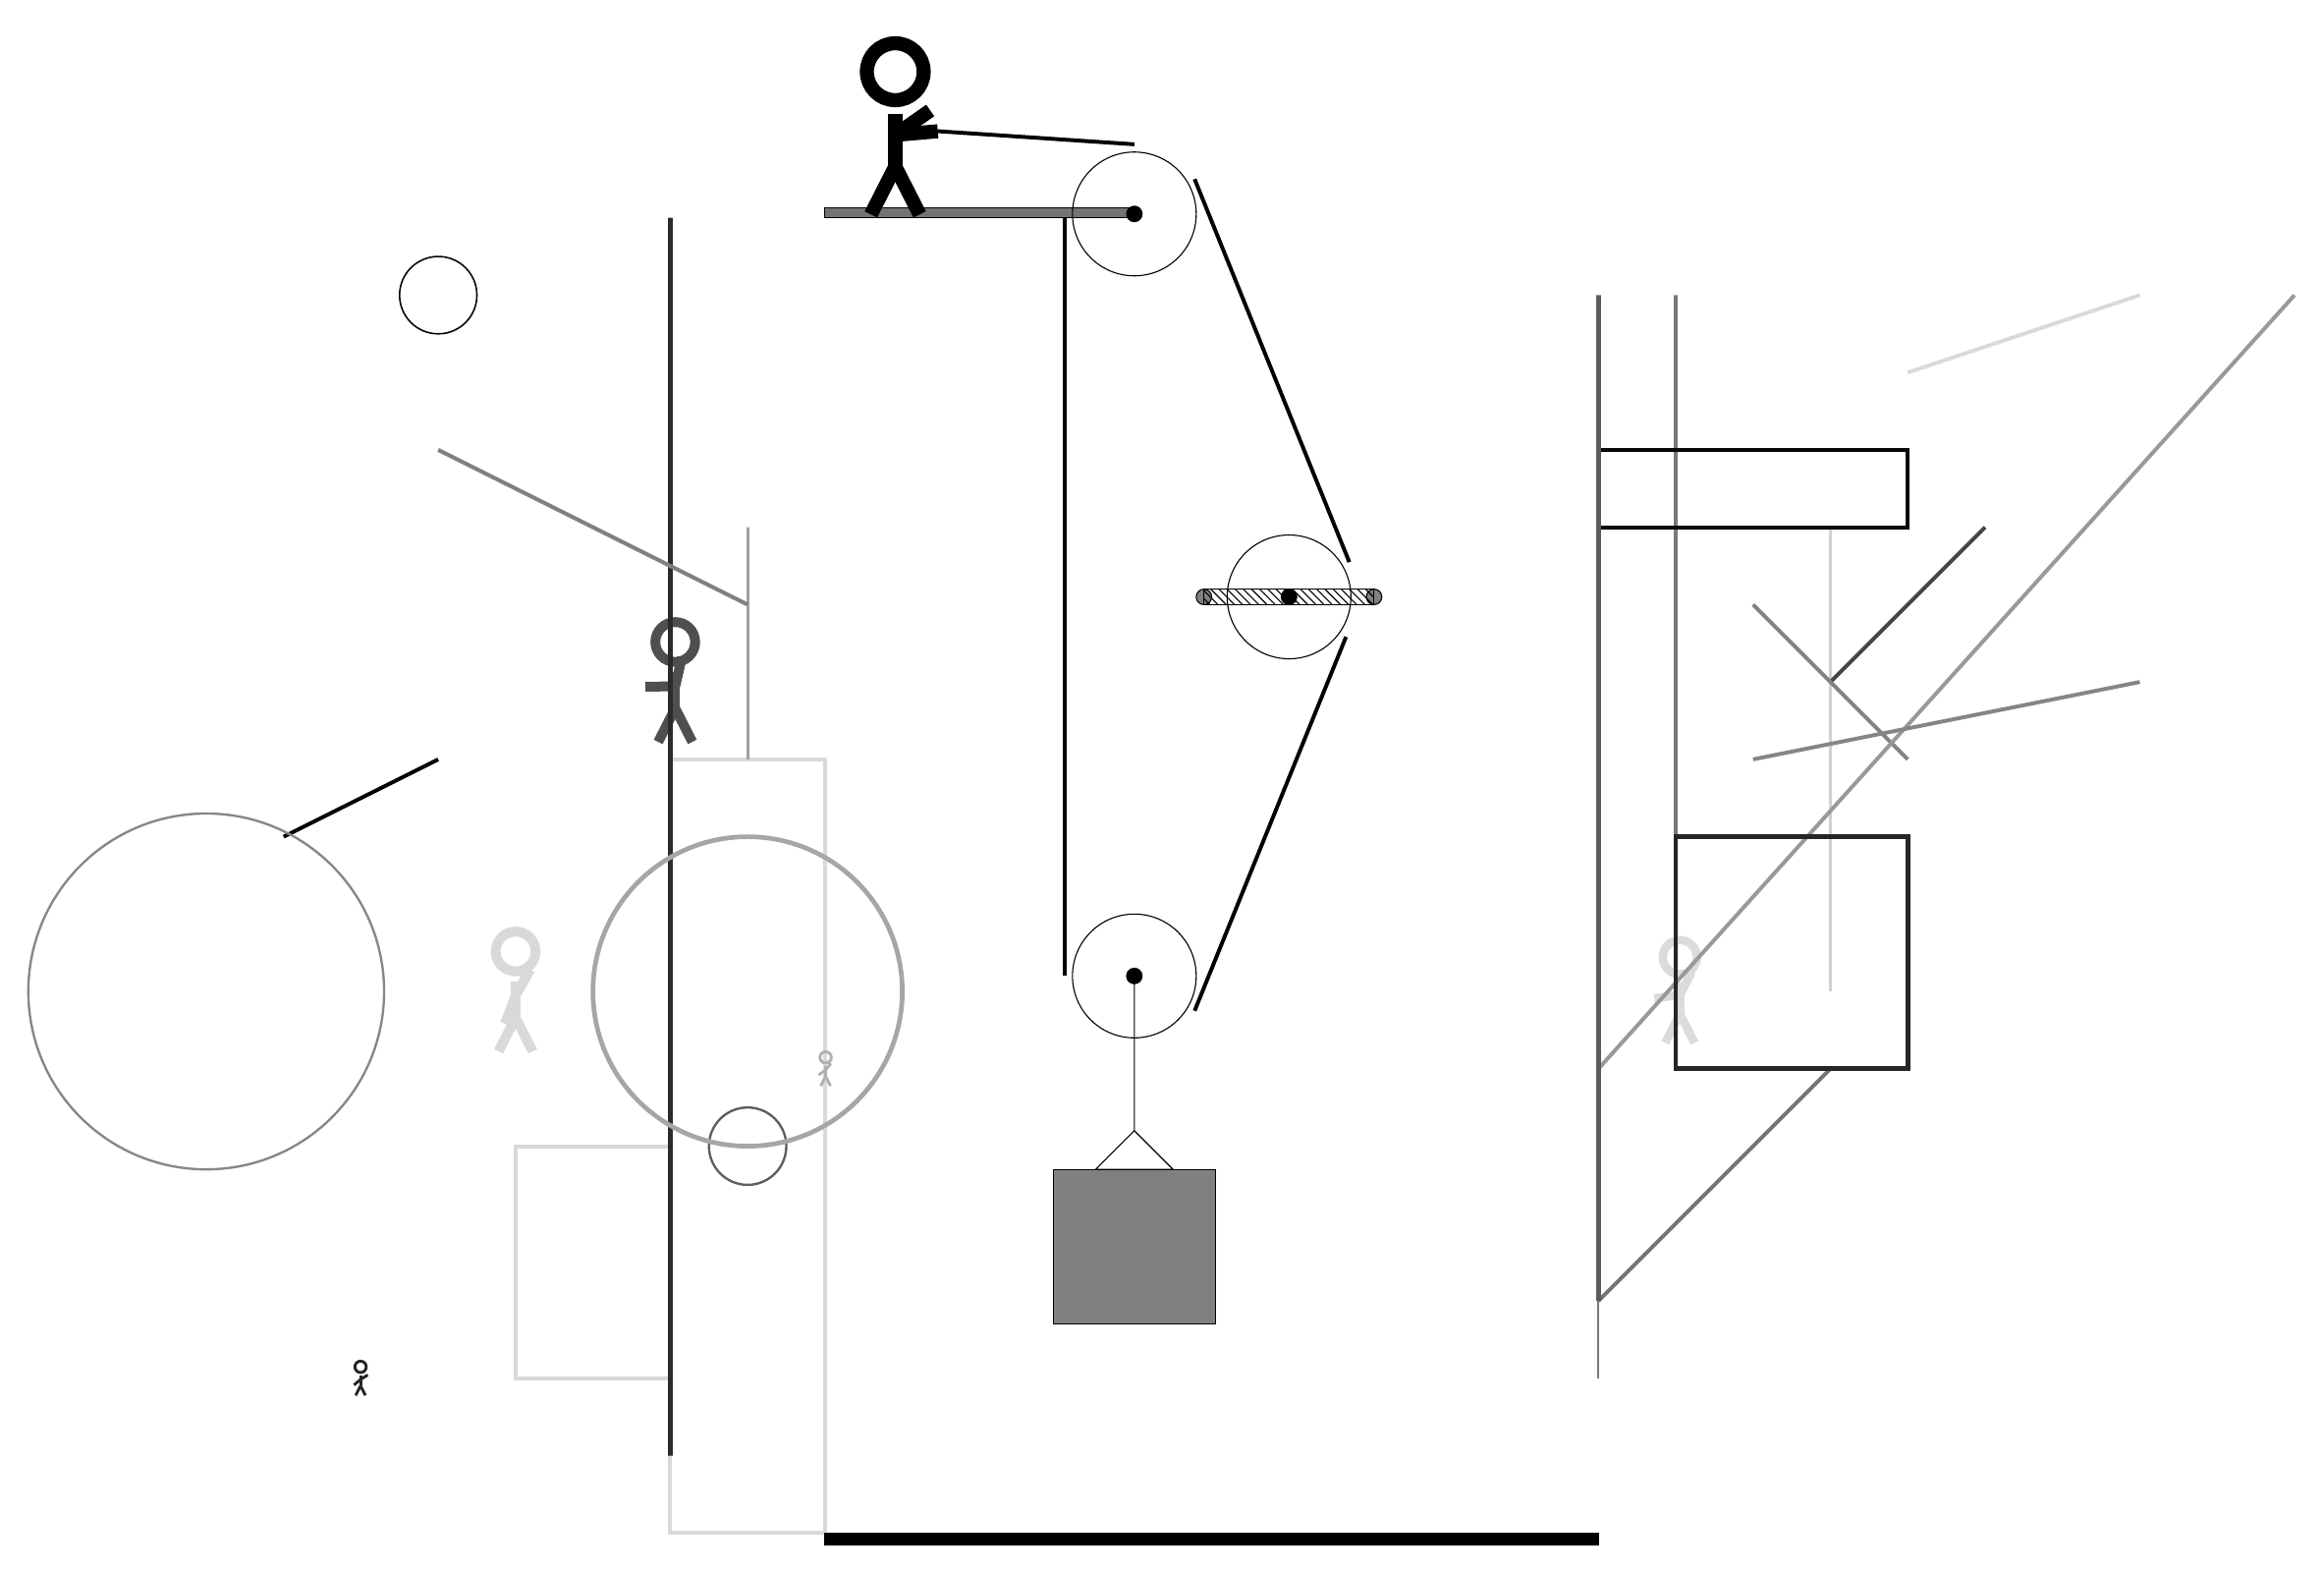
\begin{tikzpicture}
			%%%%% START %%%%%
			
			\draw[fill=black!55] (-2, 14) rectangle (2, 14.125);
			
			\draw (2, 4.2) circle (0.8);
			\draw[fill=black] (2, 4.2) circle (0.1);
			
			\draw (2, 14.05) circle (0.8);
			\draw[fill=black] (2, 14.05) circle (0.1);
			
			\draw[fill=white](4, 9.1) circle (0.8);
			\draw[fill=black] (4, 9.1) circle (0.1);
			\draw[fill=black!50] (2.9, 9.1) circle (0.1);
			\draw[fill=black!50] (5.1, 9.1) circle (0.1);
			\draw[pattern=north west lines, pattern color=black] (2.9, 9.2) rectangle (5.1, 9.0);
			
			\draw[line width=0.5mm, color=black!18](11, 4) -- (11, 10);
			
			\node[line width=0.7mm, color=black!14] at (9, 4) {\Strichmaxerl[6][7][63]};
			\draw[line width=0.5mm, color=black!54](8, 0) -- (11, 3);
			\draw[line width=0.6mm, color=black!53] (9, 13) rectangle (9, 3);
			\draw[line width=0.5mm, color=black!99](-7, 7) -- (-9, 6);
			
			\draw[line width=0.3mm, color=black!52] (8, 3) rectangle (8, -1);
			\draw[line width=0.5mm, color=black!15] (-4, -3) rectangle (-2, 7);
			\node[line width=0.3mm, color=black!69] at (-4, 8) {\Strichmaxerl[7][1][77]};
			\node[line width=0.5mm, color=black!15] at (-6, 4) {\Strichmaxerl[7][69][61]};
			
			\draw[line width=0.5mm, color=black!15] (-4, 2) rectangle (-6, -1);
			\draw [line width=0.3mm, color=black!47](-10, 4) circle (2.3);
			
			\draw[line width=0.5mm, color=black!73](11, 8) -- (13, 10);
			\draw[line width=0.7mm, color=black!83] (-4, 14) rectangle (-4, -2);
			
			\draw [line width=0.3mm, color=black!63](-3, 2) circle (0.5);
			\draw[line width=0.4mm, color=black!37] (-3, 10) rectangle (-3, 7);
			\draw[line width=0.5mm, color=black!49](10, 9) -- (12, 7);
			
			\node[line width=0.2mm, color=black!31] at (-2, 3) {\Strichmaxerl[2][35][51]};
			\draw [line width=0.6mm, color=black!85](9, 5) circle (0.0);
			\draw[line width=0.5mm, color=black!40](8, 3) -- (17, 13);
			\draw[line width=0.5mm, color=black!48](10, 7) -- (15, 8);
			\node[line width=0.5mm, color=black!86] at (-8, -1) {\Strichmaxerl[2][40][32]};
			\draw[line width=0.5mm, color=black!97] (8, 11) rectangle (12, 10);
			
			\draw [line width=0.2mm, color=black!98](-7, 13) circle (0.5);
			\draw[line width=0.5mm, color=black!50](-3, 9) -- (-7, 11);
			\draw[line width=0.5mm, color=black!15](12, 12) -- (15, 13);
			
			\draw[line width=0.6mm, color=black!85] (9, 6) rectangle (12, 3);
			
			\draw [line width=0.6mm, color=black!35](-3, 4) circle (2.0);
			\draw[line width=0.6mm, color=black!64] (8, 0) rectangle (8, 13);
			
			
			\draw (2, 4.2) -- (2, 2.2) -- (1.5, 1.7) -- (2.5, 1.7) -- (2, 2.2);
			\draw[fill=black!50] (0.95, 1.7) rectangle (3.05, -0.3);
			
			\draw[line width=0.5mm] (1.1, 14) -- (1.1, 4.2);
			\centerarc[line width=0.5mm](2, 4.2)(180:330:0.9);
			\draw[line width=0.5mm](2.7794, 3.75) -- (4.7373, 8.5838);
			\centerarc[line width=0.5mm](4, 9.1)(390:325:0.9);
			\draw[line width=0.5mm](4.7794, 9.55) -- (2.7794, 14.5);
			\centerarc[line width=0.5mm](2, 14.05)(30:90:0.9);
			\draw[line width=0.5mm](2, 14.95) -- (-1, 15.15);
			
			\node at (-1, 15.15) {\Strichmaxerl[10][-175][35]};
			
			\draw[fill=black] (-2, -3) rectangle (8, -3.15);
			
			%%%%% END %%%%%
		\end{tikzpicture}
	\end{figure}	
\end{document}